\chapter{Deep Multi-Agent RL Experiments}
All of the methods discussed in this work are typically implemented in function approximation
settings.
Hence, it is important to evaluate if the observed performance improvements carry over when the
policy parameters, and the value approximation are both represented using neural networks.

Expanding on our the observations from the tabular experiments, we proceed to evaluate the
algorithms in large-scale 2p0s games to answer question~\ref{qn3}.
For the neural experiments, we study the effect of the NeuRD-fix, and the utilization of
Optimistic-variants of popular optimizers (Optimistic-SGD, and Optimistic-Adam) when paired with
deep RL algorithms.
% Extragradient updates require more orchestration when learning through self-play, are more
% restrictive in how the training is performed.
% Hence, we do not study the EG variants in this section.

\section{Experimental Domains}
For these experiments we choose three 2p0s EFGs, namely - Kuhn Poker, Abrupt Dark Hex, and Phantom
Tic-tac-toe.
Please refer to Appendix~\ref{apx:gamedesc} for a description of these games.

We train all the algorithms through self-play reinforcement learning.

\section{Evaluation Metrics}
The measures used in tabular experiments are harder to compute for large-scale EFGs.
Distance to an equilibrium point is harder to compute due to the absence of a unique equilibrium
point.
For larger games, the computation of exact best responses to measure the exact exploitability is
prohibitive due to the large state space.
However, we can approximate the exploitability computation if we can approximate the best response
for a given fixed policy.

\subsection{Approximate Exploitability}
We can learn a local best response by training a best response agent against the fixed policy we
wish to evaluate~\cite{timbersApproximate2022}.
Then the exploitability can be approximated by sampling trajectories and measuring the average
reward the best response agent acheived against the exploited policy.
In our experiments, we train the best response agent against the fixed joint-policy learn through
self-play.
Let $\pi_{BR}$ be a learnt best-response approximator, and $\pi_{fixed}=(\pi_1, \pi_2)$ be the
joint policy to be exploited, then the approximate exploitability is given by:
\begin{equation}
	\label{eqn:appxexp} \text{Exp}_{appx} (\pi_{BR}, \pi_{fixed}) = \frac{1}{N} \left[ \sum_{i=1}^{N/2}
		\E_{a \sim \pi_1, \pi_{BR}} [R] + \sum_{i=1}^{N/2} \E_{a \sim \pi_{BR}, \pi_2} [R] \right]
\end{equation} \fillin{TBD: rephrase the equation in terms of cumulative episodic rewards.
}

\section{Experiment Setup}
Due to the strong performance exhibited by MMD~\cite{sokotaUnified2023} as a deep MARL algorithm
for 2p0s games, we consider vanilla-MMD to be our baseline.
For a fair comparison of all the algorithms, we setup our experiments
following~\cite{sokotaUnified2023}, by implementing MMD as a modification of
RLLib's~\cite{liangRLlib2018} PPO implementation.
We use OpenSpiel's~\cite{lanctotOpenSpiel2020} game implementations and use RLLib's environment
adapter to interact with OpenSpiel.

For all the experiments we a use 2-layered MLP with (128, 128) hidden units for the policy and the
value networks without shared parameters.
We note that RLLib's implementation makes use of Generalized Advantage Estimates
(GAE)~\cite{schulmanHighDimensional2018} instead of regular advantage estimates, and we retain that
choice for our experiments as well.
For all the experiments, we learn an approximate best-response agent by training a DQN agent
against the fixed joint-policy to compute approximate exploitability.
% We use GAE for computing the advantage estimates.% Please refer to the table~\ref{tab:hpes} in the appendix for a more exhaustive list of% hyperparameter values.
For the smaller games (Kuhn Poker, and Abrupt Dark Hex 2$\times$2), we train the agents in
self-play for 1M steps and report exact exploitability across the training iterations.
We also train the DQN agent for 1M steps against the fixed joint-policy obtained at the end of
training to compute the approximate exploitability.
For Abrupt Dark Hex 3$\times$3, and Phantom TTT we train the agents for 5M steps and only report
the approximate exploitability of the final joint-policy by training the DQN agent for 5M steps.
For all approximate exploitability evaluations, we evaluate the agents for $N=1000$ episodes with
the DQN agent starting first in 500 episodes, and the exploitee agent starting first in 500
episodes.

\section{Results}
\ref{fig:neuralsmall1} plots the exact exploitabililty of the joint policy as a function of the
iterations, and~\ref{fig:neuralsmall1} shows the approximate exploitability at the end of training for these games.
These results show correspondence between exact and approximate exploitability as expected
qualifying the latter as a valid evaluation metric for the larger games.
In agreement to the tabular experiments, the NeuRD versions of these algorithms have a better
performance.

\begin{figure}[H]
	\centering
	\begin{subfigure}[b]{0.6\textwidth}
		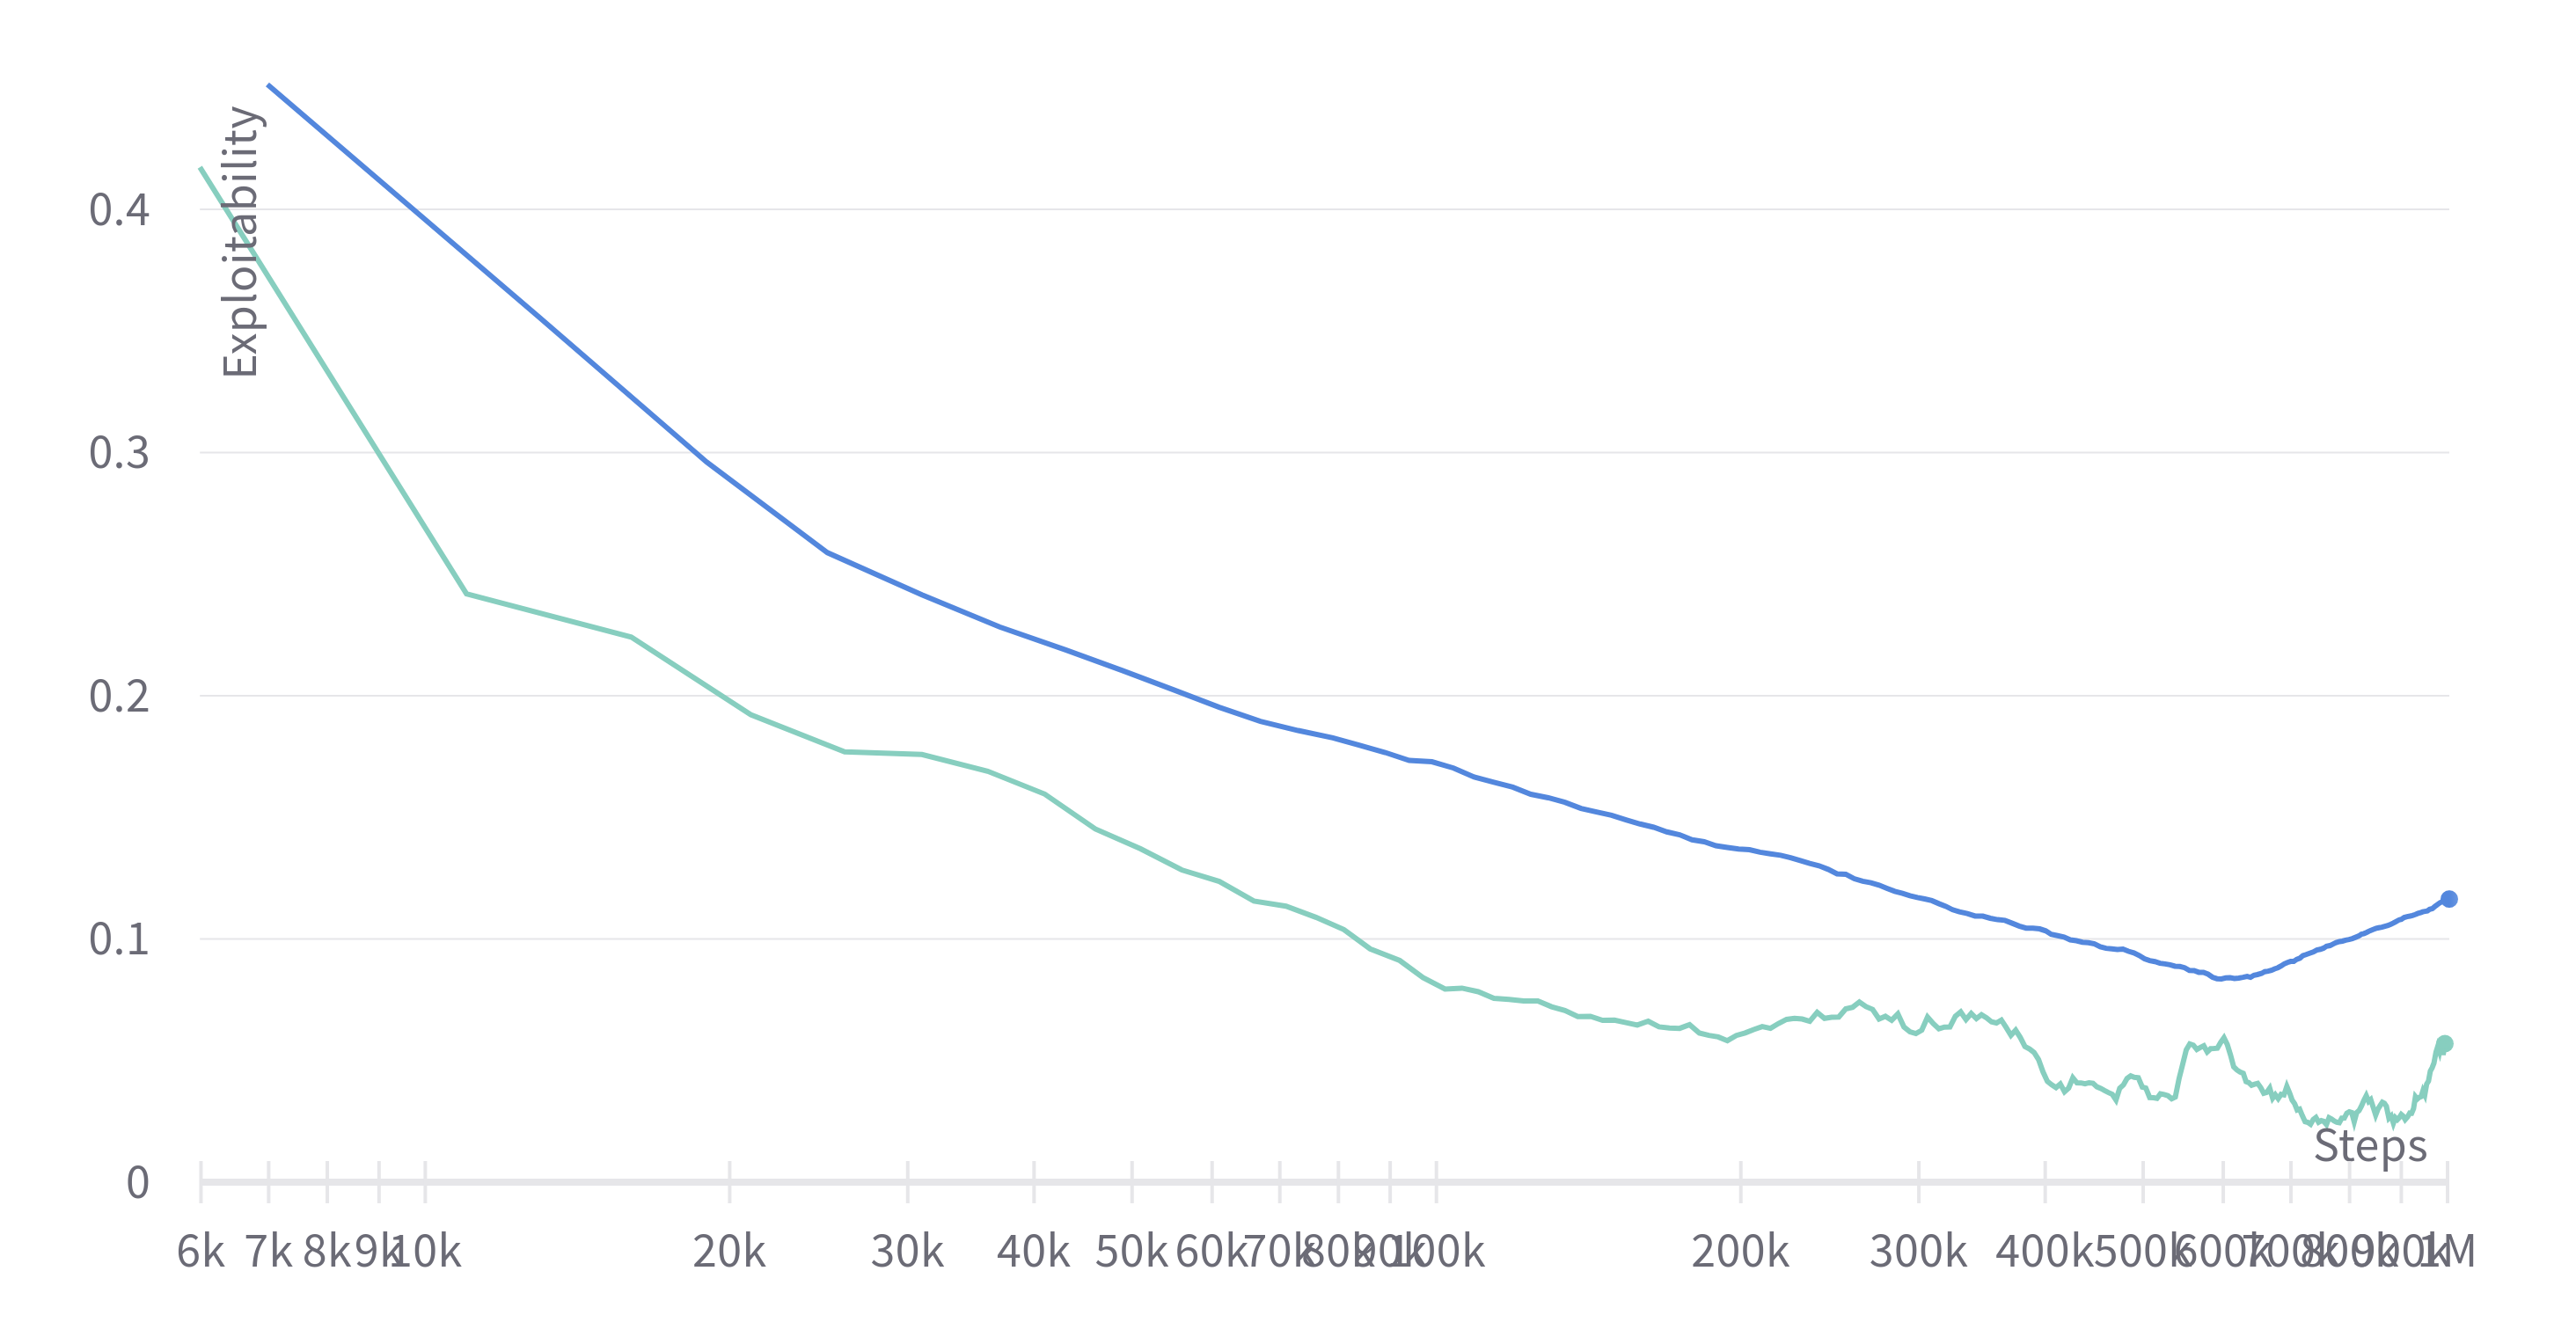
\includegraphics[width=\textwidth]{figs/kpoker.png}
		\caption{Kuhn Poker}
	\end{subfigure}
	\begin{subfigure}[b]{0.6\textwidth}
		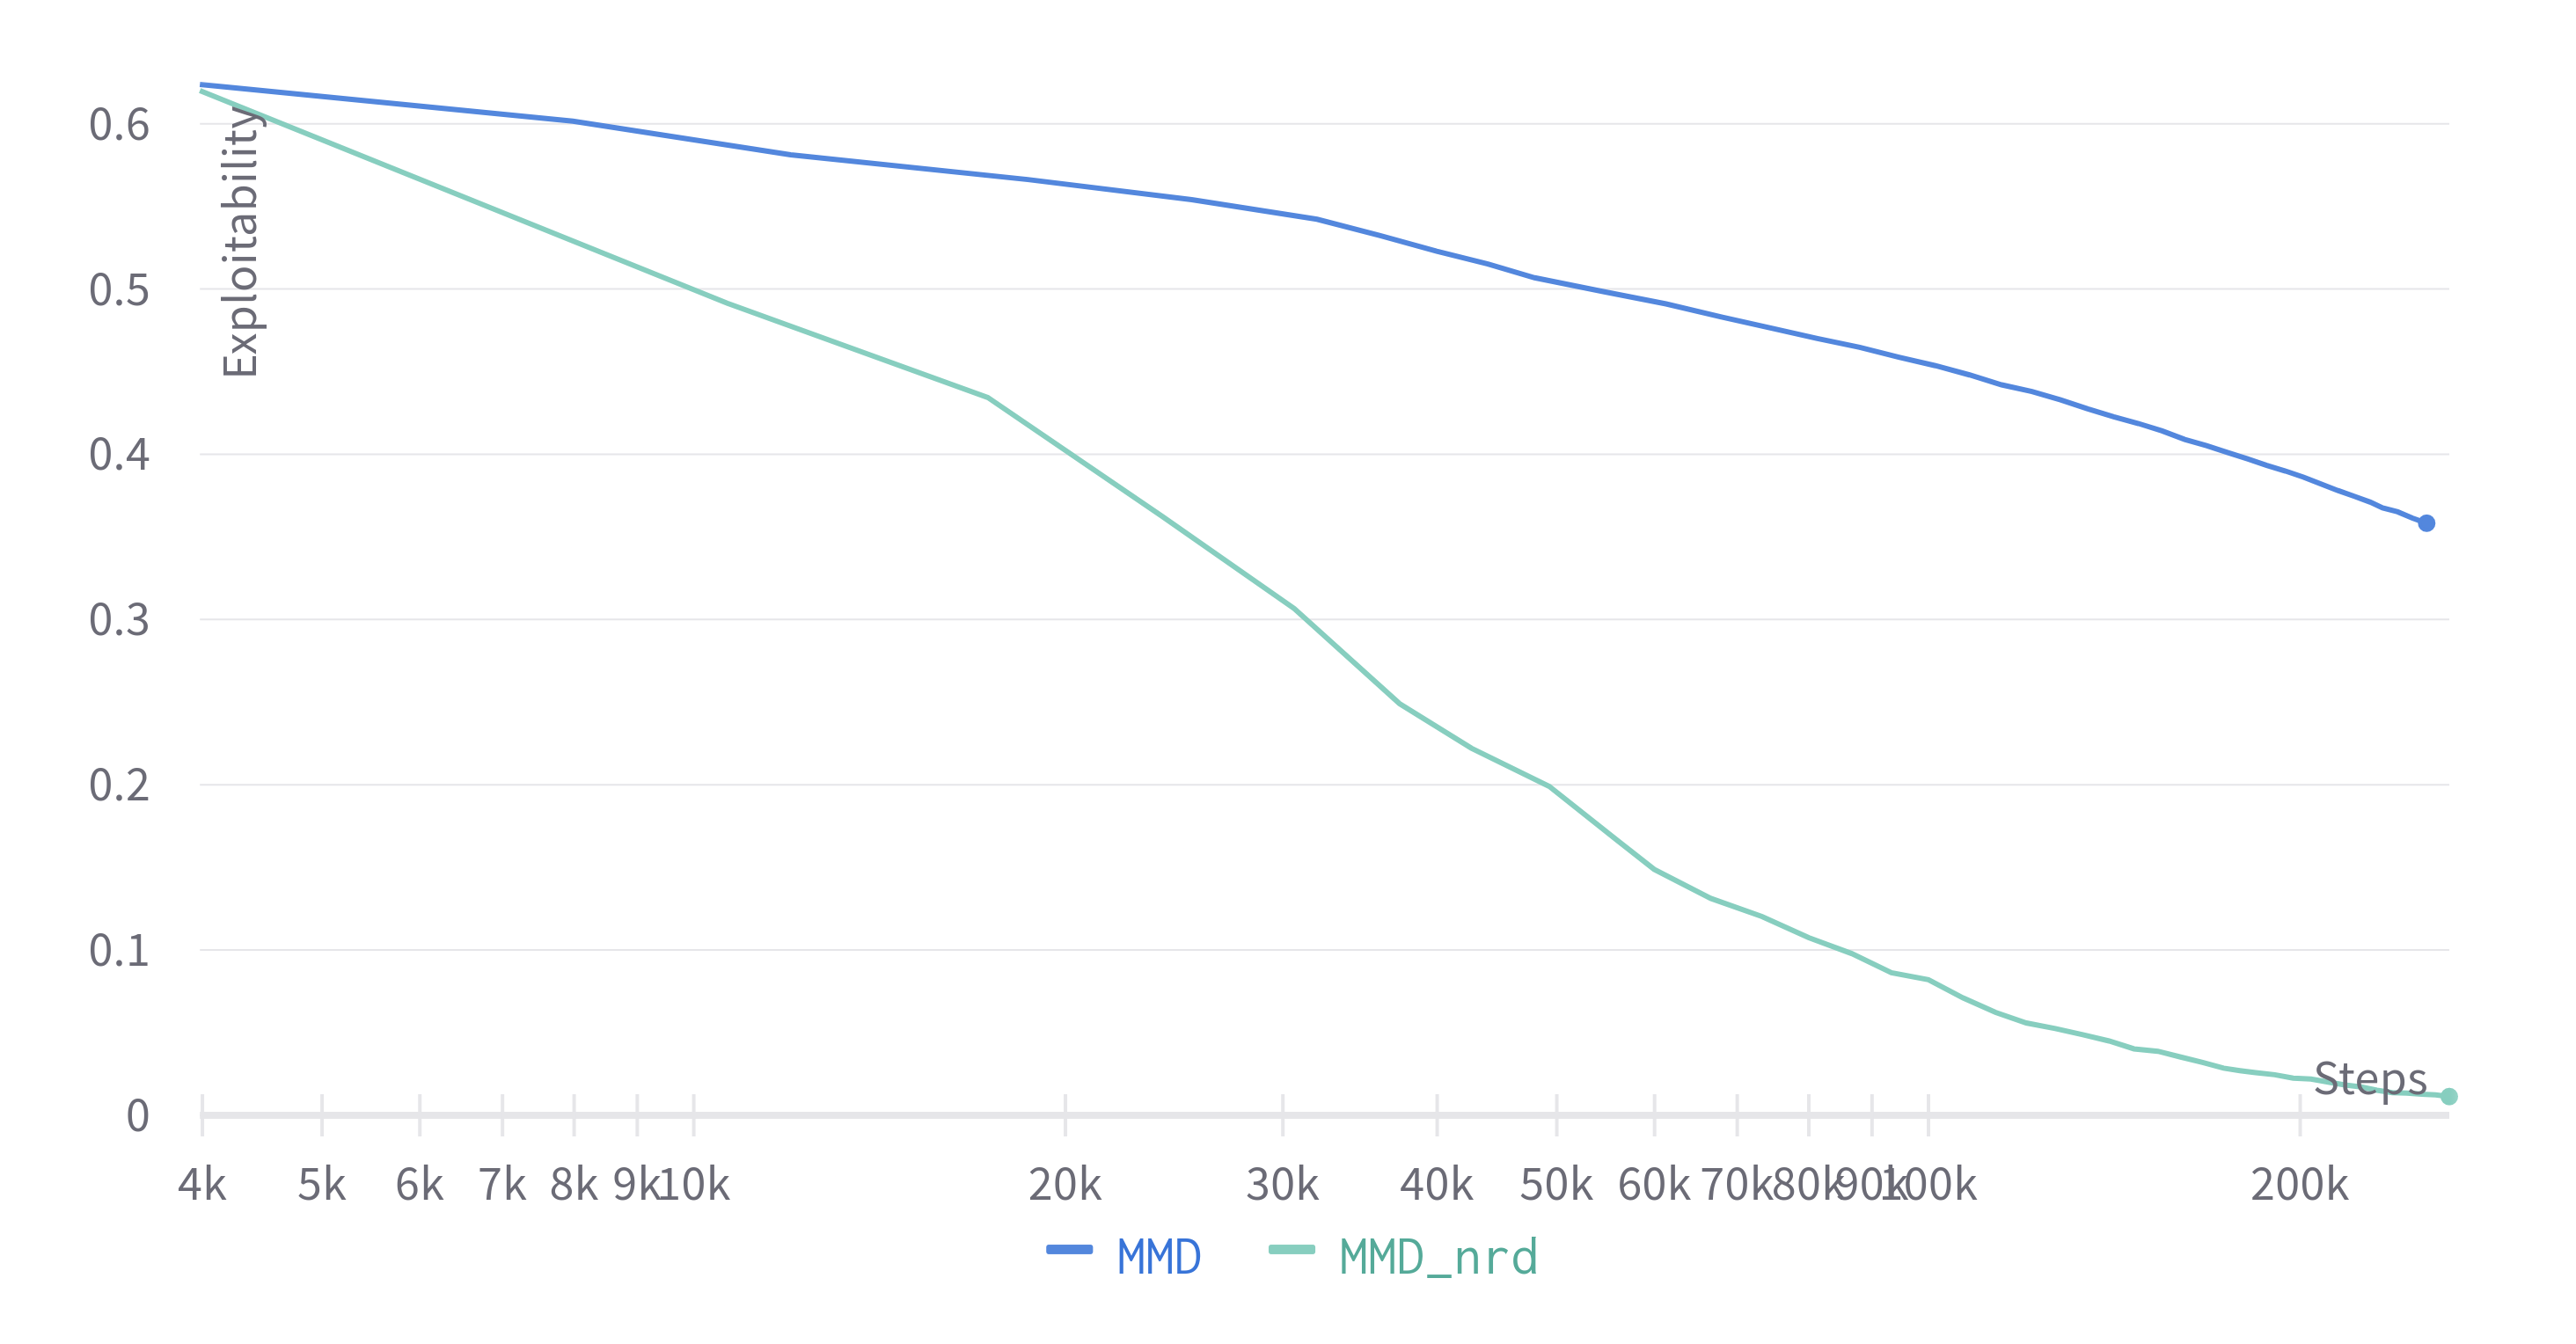
\includegraphics[width=\textwidth]{figs/ahex22.png}
		\caption{Abrupt Dark Hex (2$\times$2) (\red{1M steps version to be added})}
	\end{subfigure}
	\caption{Performance in small EFGs, measured by exact exploitability.}
	\label{fig:neuralsmall1}
\end{figure}

% We also compute approximate exploitability for the smaller games by training a DQN best-response
% agent for 1M steps against the fixed trained agents.

\ref{fig:neural2} shows improvement in performance by applying the NeuRD-fix in Abrupt Dark Hex
(3$\times$3) and Phantom TTT, as measured by the approximate exploitability.
\begin{figure}[H]
	\centering
	\begin{subfigure}[b]{0.4\textwidth}
		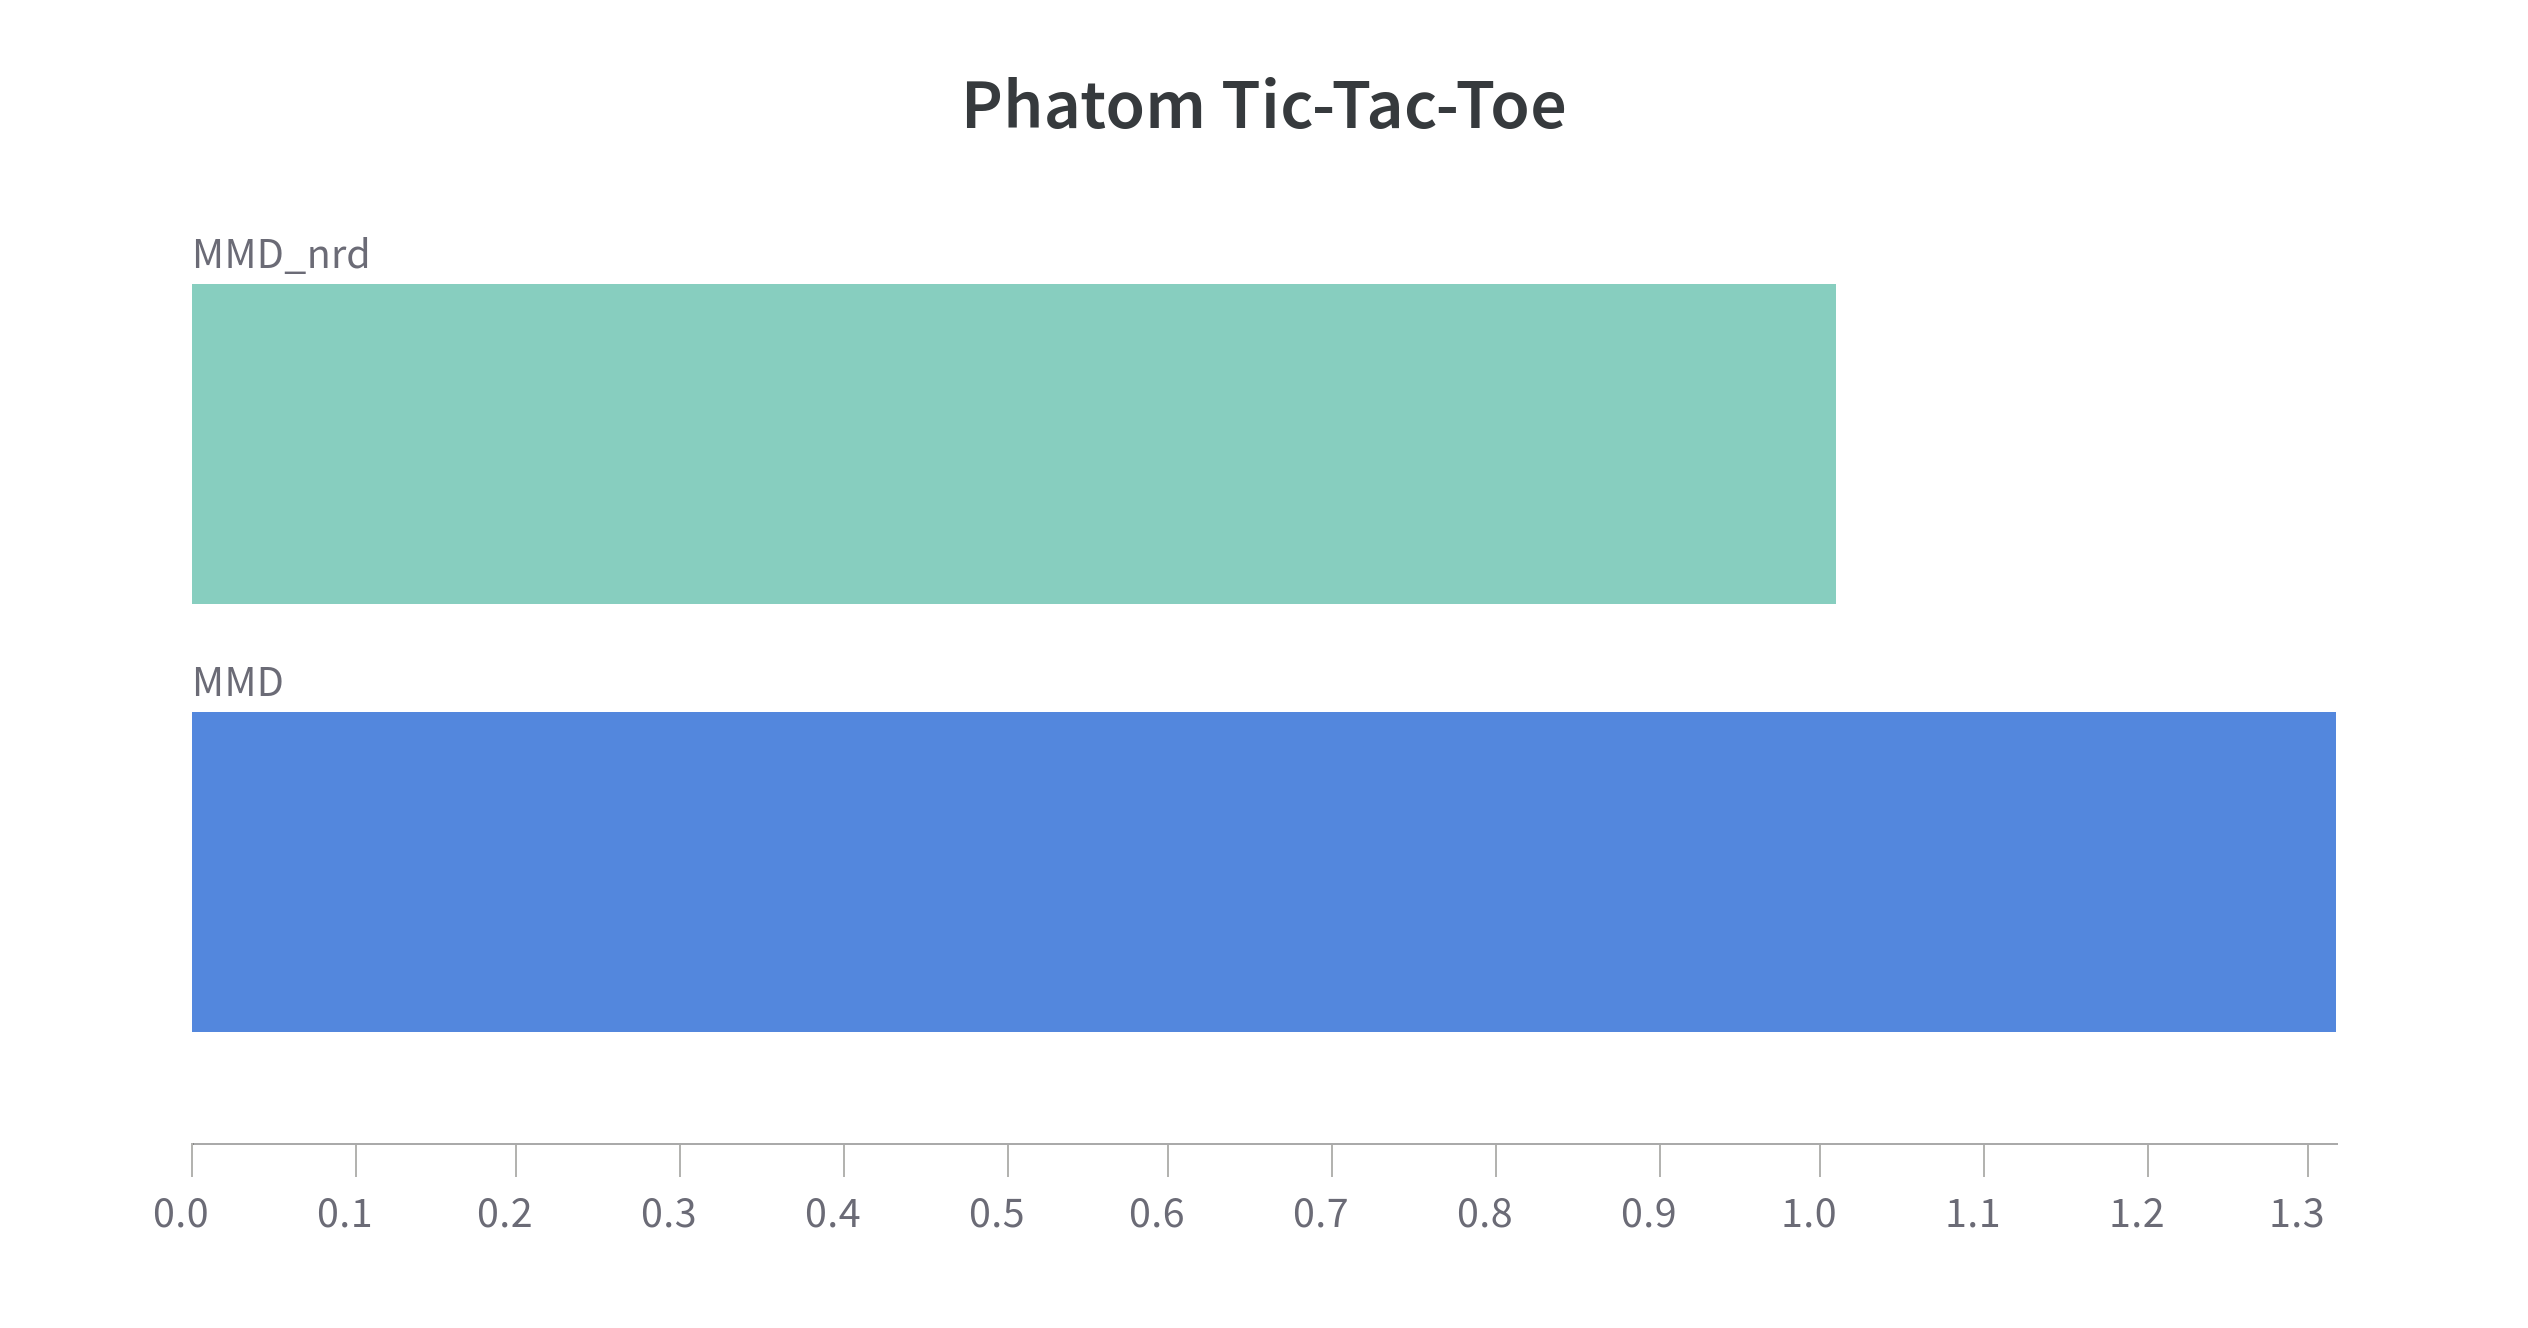
\includegraphics[width=\textwidth]{figs/pttt.png}
		\caption{Kuhn Poker}
	\end{subfigure}
	\begin{subfigure}[b]{0.4\textwidth}
		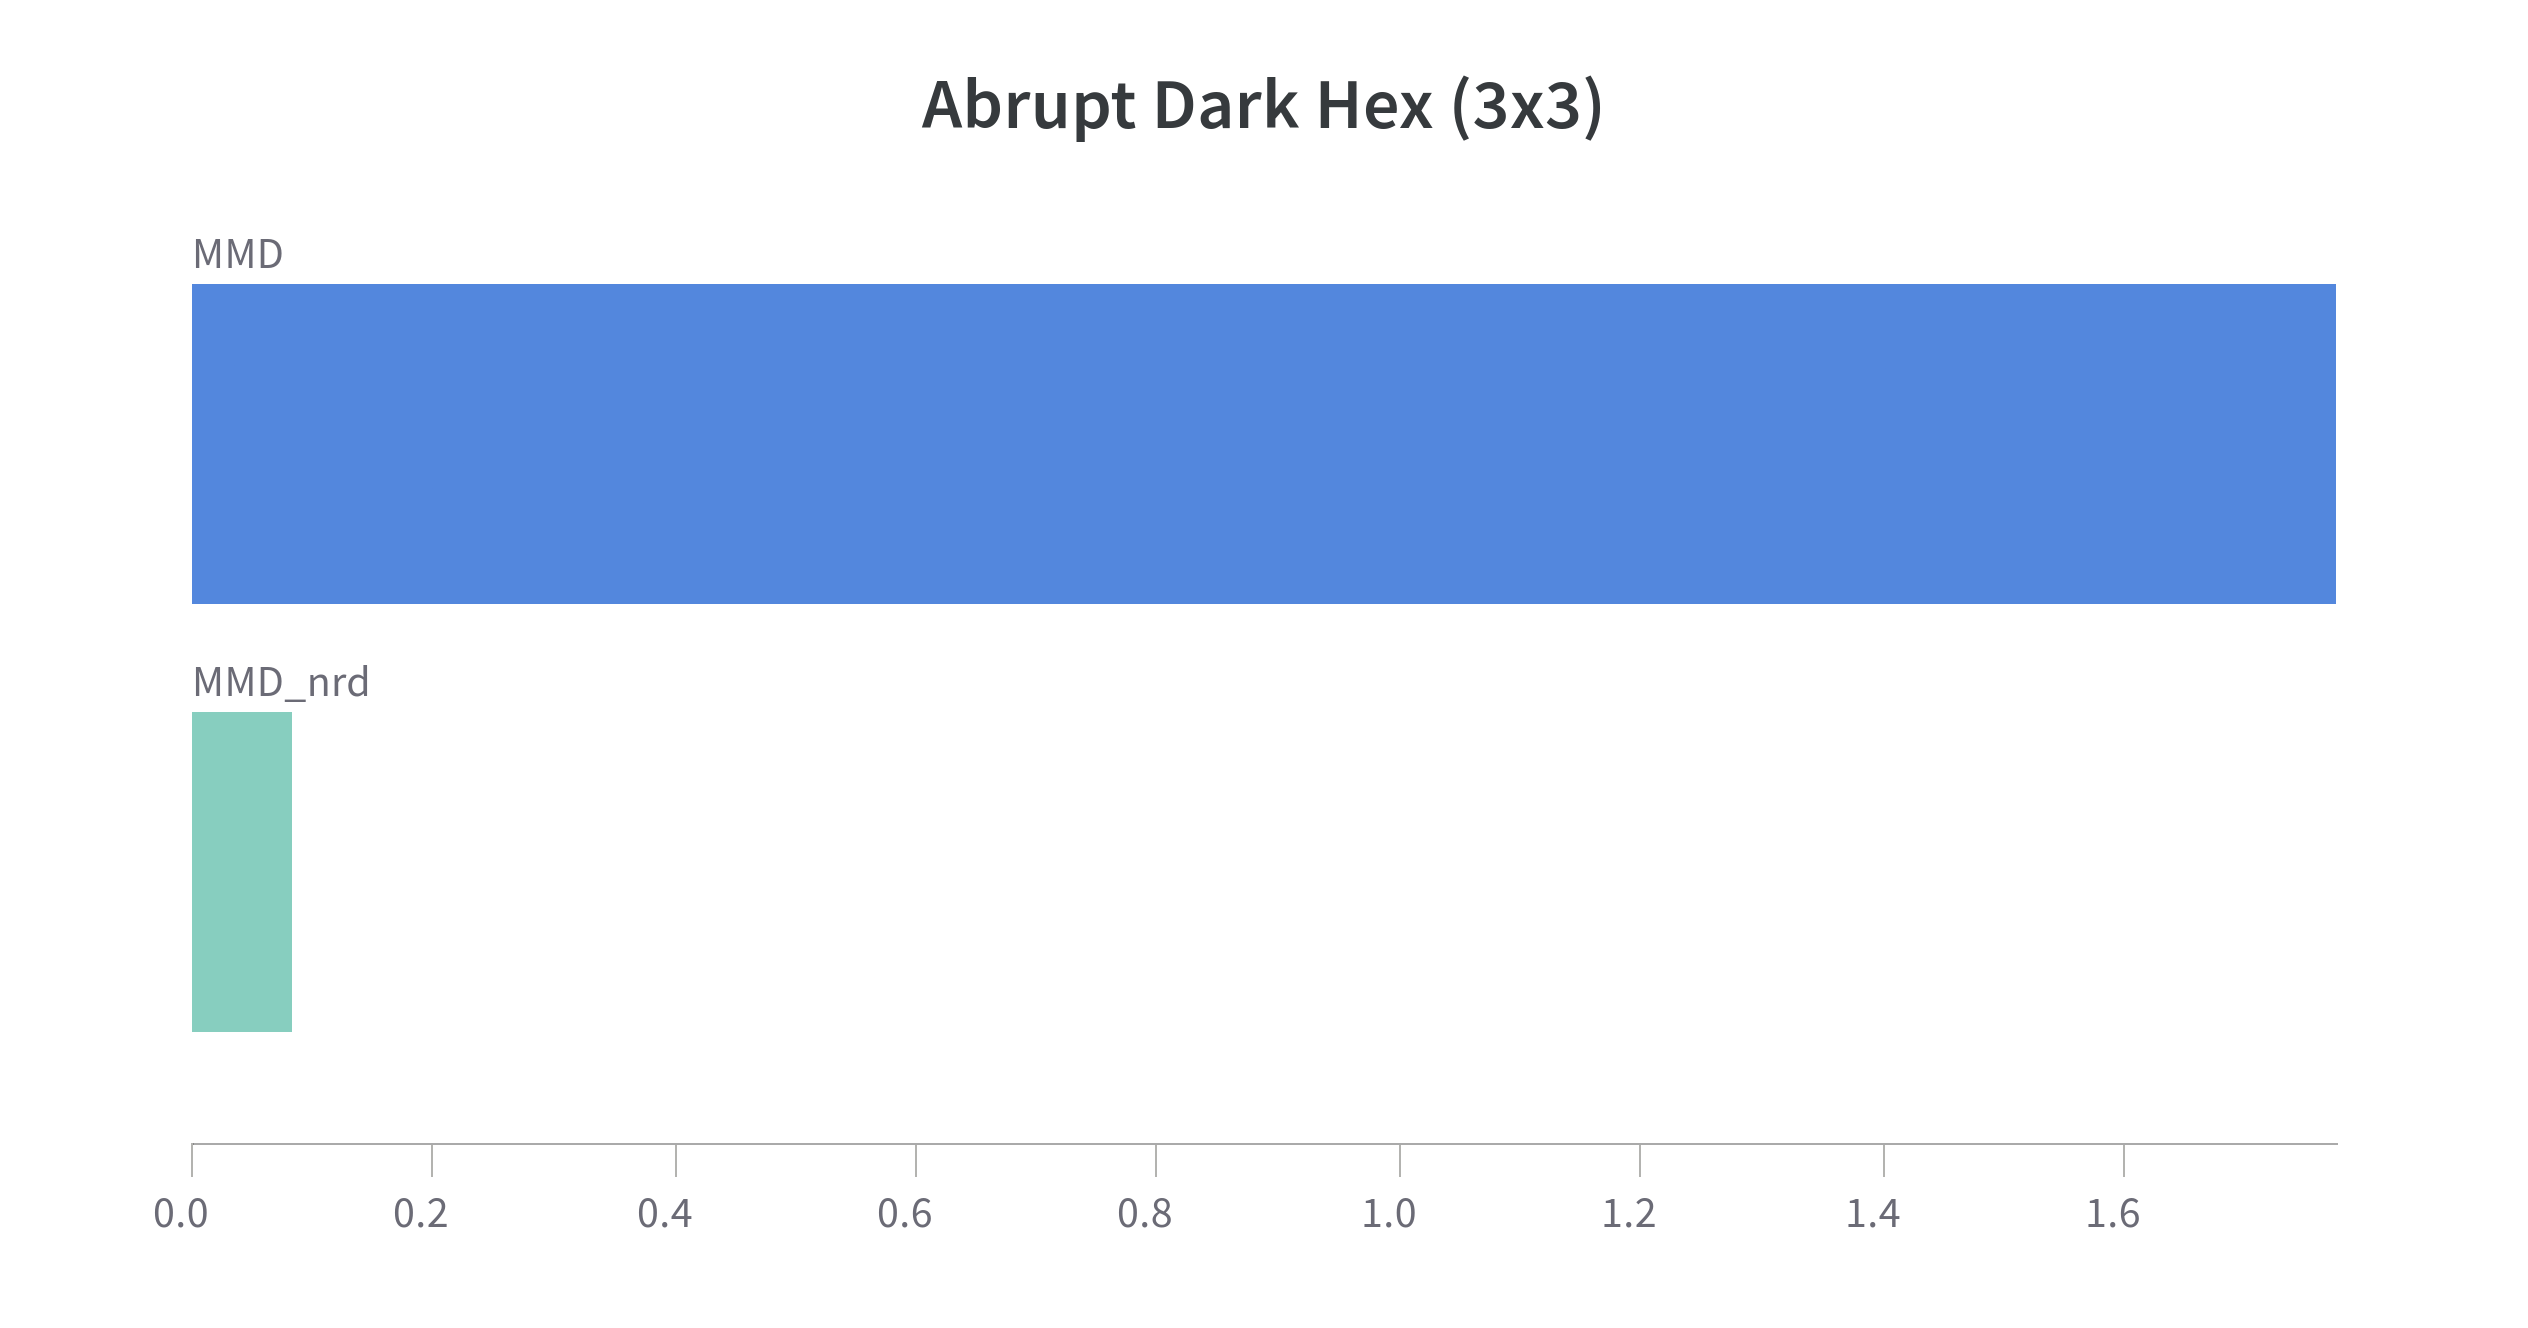
\includegraphics[width=\textwidth]{figs/ahex33.png}
		\caption{Abrupt Dark Hex (3$\times$3)}
	\end{subfigure}
	\caption{Performance in larger EFGs, measured by approximate exploitability.}
	\label{fig:neural2}
\end{figure}

\fillin{We also evaluate these algorithms by having the trained agents play against each other in a
	head-to-head manner.}